

% This is based on the LLNCS.DEM the demonstration file of
% the LaTeX macro package from Springer-Verlag
% for Lecture Notes in Computer Science,
% version 2.4 for LaTeX2e as of 16. April 2010
%
% See http://www.springer.com/computer/lncs/lncs+authors?SGWID=0-40209-0-0-0
% for the full guidelines.
%
\documentclass{llncs}
\usepackage[utf8]{inputenc}
\usepackage[ngerman]{babel}
\usepackage{graphicx}
\usepackage{hyperref}
\usepackage{listings}
\usepackage{hyperref} 

\begin{document}
\title{HTTP und HTTP/2}
\author{Michael Hochleitner}
\institute{Ludwig-Maximilians-Universit\"at M\"unchen}

\maketitle 
\begin{center}
Bachelorseminar ``Web Technologies'' \\
Wintersemester 2017/18
\end{center}

\begin{abstract}
HTTP ist ein Netzwerkprotokoll, das benutzt wird um Datenpakete zwischen Rechnern in Rechnernetzen auszutauschen. Es ist ein Request-Response-Protokoll. Die Datenpakete sind entweder Anfragen oder Antworten. Die erste Version HTTP/0.9 wurde 1990 entwickelt. Seitdem wurde das Protokoll in mehreren Protokollversionen erweitert. HTTP/1.0 bietet Metadaten über den Paketinhalt, mehrere Methoden, um verschiedene Absichten des Clients auszudrücken  und Statuscodes.
Ein Schwerpunkt bei den Erweiterungen des Protokolls ist Performanz. Verbesserungen in der Performanz erreicht man durch effiziente Nutzung des unterliegenden Transportprotokolls. HTTP/1.1 erlaubt Pipe\-lining von mehreren Anfragen auf einer TCP-Verbind"-dung. Beim Pipe\-lining tritt das Problem HOL-Blocking auf. Das wird in \mbox{HTTP/2} durch Multiplexing umgangen.  Die prominenteste Anwendung, die HTTP nutzt, ist das World Wide Web, das auf dem Internet aufsitzt.
\keywords{Protokoll, Rechnernetze, Internet, World Wide Web, Hypertext, HTTP, HTTP/2}
\end{abstract}

\section{Einleitung}
In der Forschungseinrichtung CERN in Genf arbeiteten in den 90er Jahren viele Leute, die verschiedene Betriebssysteme und verschiedene Textverarbeitungsprogramme benutzten, um ihre Ergebnisse zu dokumentieren. Der Austausch von digitalen Dokumenten war schwierig. Deshalb entwickelte der Informatiker Tim Berners-Lee ein Dokumentationssystem. \cite{Berners-Lee1999}

Das Dokumentationsystem baut auf den Technologien Internet, Hypertext und dem Aufrufen von Prozeduren auf anderen Computern, genannt RPC (Remote Procedure Call) auf. Es wurde bekannt unter dem Namen World Wide Web. Die Architektur des World Wide Web ist Client-Server. Der Client sollte ein Programm sein, mit dem man Hypertextseiten erstellen, durchblättern und editieren kann. Der Server sollte ein Programm sein, das die Hypertextseiten hält und den Benutzern des World Wide Web Zugriff darauf erlaubt.\cite{Berners-Lee1999}


Durch das gemeinsame Dateiformat HTML (Hypertext Markup Language), die Verbindung von Computern über das Internet und das Abspeichern der HTML-Dateien auf einem Server, wurde der Zugriff auf digitale Dokumente von Computern mit unterschiedlichen Betriebssystemen möglich.

Um Dateien auf einem Server für andere Computer zur Verfügung zu stellen, versendet man die Dateien in Datenpaketen. Dafür benötigt man ein Protokoll. Das Protokoll des World Wide Web ist HTTP, das Hypertext Transfer Protocol.
\section{HTTP Grundlagen}
In diesem Kapitel werden die Spezifikationsdokumente für HTTP vorgestellt, es gibt eine Versionsübersicht und es werden einige grundlegende Eigenschaften des Protokolls anhand der Version 0.9 erläutert. 

HTTP gibt es in vier Versionen. Die Versionsnummern sind 0.9, 1.0 1.1 und 2. Definiert wird HTTP in Requests for Comments (RFCs), die von der Internet Engineering Task Force (IETF) und der Internet Society (ISOC) herausgegeben werden. RFCs sind Dokumente, die öffentliche Standards zu Internettechnologien vorschlagen.

Die Versionsnummer 0.9 ist die Versionsnummer des ersten Prototypen von HTTP. 1.0 ist die erste Versionsnummer, die in einem RFC veröffentlich wurde. Der RFC 1945 beschreibt HTTP 1.0, der RFC 2616 beschreibt HTTP 1.1 und der RFC 7540 beschreibt HTTP 2.0.
Der RFC 2616 ist die erste standardisierte Spezifikation von HTTP.


Mit HTTP/0.9 kann man Datenpakete über eine TCP Verbindung verschicken. Das Protokoll definiert welche Form die Datenpakete haben müssen, damit Client und Server kommunizieren können. Es unterscheidet zwei Arten von Datenpaketen: Anfragen und Antworten. Anfragen werden vom Client an den Server geschickt. Antworten enthalten bei einer erfolgreichen Anfrage die angefragte Datei. Um eine HTML Datei zu empfangen, muss ein Client über eine TCP-Verbind"-dung eine Anfrage schicken. In der Anfrage wird die Datei, die übertragen werden soll spezifiziert. Es folgt ein Beispiel für eine Anfrage.

\lstset{ 
  basicstyle=\ttfamily, frame = single
}
\begin{lstlisting}[caption={HTTP GET-Anfrage},label={lst:get}]
GET /index.html
\end{lstlisting}

Die Methode in Listing \ref{lst:get} ist GET. Sie bedeutet, dass eine Datei vom Server zum Client übertragen werden soll. Der Server, die IP-Adresse und der Port müssen in HTTP-Anfragen nicht spezifiziert werden. Das ist Aufgabe der unterliegenden Protokolle IP und TCP. Die GET-Methode bekommt als Parameter einen URI. Der URI ist die Adresse der Datei. Die Datei nennt man auch Ressource.

Wenn eine Anfrage bei einem Server ankommt, muss er entscheiden, ob er die angeforderte HTML-Datei verschicken kann. Wenn er das kann ist die Antwort in der Protokollversion 0.9 die angefragte HTML-Datei. Der RFC 2616 bezeichnet das als "`raw data transfer'' \cite{Fielding1999}.

Aufgrund des Anfrage-Antwort-Mechanismus, den HTTP nutzt, wird es der Gruppe der Request-Response-Protokolle zugeordnet. Die Codierung für die Protokollversionen 0.9, 1.0 und 1.1 ist ASCII. Das ist so, weil die Mindestanforderungen an einen Computer, der über HTTP kommunizieren sollte, möglichst gering sein sollten. Es wurde nur vorrausgesetzt, dass der Computer eine Tastatureingabe hatte und ASCII-Zeichen produzieren konnte \cite{Berners-Lee1999}.

Die HTTP Version 0.9 eignet sich gut, um den Request-Response-Charakter von HTTP anschaulich darzustellen, weil die Anfragen und Antworten sehr kompakt sein können. Listing \ref{lst:html} zeigt ein Beispiel für eine Antwort, die mit HTTP 0.9 konform ist.

\begin{lstlisting}[caption={Antwort-Paket nach HTTP 0.9},label={lst:html}]
<html>
<p>Das ist eine HTML-Datei.<\p>
</html>
\end{lstlisting}

\section{Methoden}
Der wichtigste Bestandteil eines HTTP-Pakets ist die Methode. Ein Datenaustausch zwischen Client und Server geht normalerweise vom Client aus. Der schickt ein Paket, das eine Methode enthält. Sie sagt dem Server was der Client will. In Kapitel 2 wurde die GET-Methode beschrieben. Die beiden wichtigsten Methoden sind GET und HEAD. Sie müssen von allen HTTP-Servern unterstützt werden \cite{Fielding1999}. Außerdem gibt es OPTIONS, POST, PUT, DELETE, TRACE und CONNECT. 

\begin{itemize}  
\item HEAD fragt Metadaten über eine Ressource ab, ohne sie zu übertragen. Die Antwort auf eine Anfrage mit der Methode HEAD enthält Headerfelder ohne den zugehörigen Paketinhalt.
\item PUT bedeutet, dass der Paketinhalt unter der angegebenen URI auf dem Server gespeichert werden soll. 
\item POST gibt eine übergeordnete URI an, unter der der Paketinhalt der Anfrage gespeichert werden soll. So wie man auf einem Dateisystem eine Datei in einem Ordner speichert. Die neue URI des Paketinhalts, der auf dem Server gespeichert wurde, wird in einer Antwort vom Server zurückgeschickt. Das ist eine Anwendungsmöglichkeit einer POST-Anfrage. Man kann mit einer POST-Anfrage auch Daten aus einem Formular an einen Prozess auf dem Server leiten, der die Daten weiterverarbeitet. Dieser Prozess kann die Daten aus dem Formular z.B. an eine Email-Adresse schicken.
Die Gemeinsamkeit aller POST-Anfragen ist, dass der Paketinhalt vom Server weiterverarbeitet wird.
\end{itemize}
Die Definitionen der anderen Methoden kann man im RFC 2616 nachlesen.
\section{Header}
Während man mit dem HTTP-Protokoll in der Version 0.9 nur HTML-Dateien
verschicken konnte, ist es ab der Protokollversion 1.0 auch möglich andere
Dateitypen zu verschicken. Der Dateityp der verpackten Datei wird im Paket
vermerkt. Diese Metadaten sind im Header.

Der Header eines Pakets besteht aus einem oder mehreren Headerfeldern.
Die Aufteilung in Metadaten und Pakethinhalt führt dazu, dass ein Antwort-Paket nach Protokollversion 1.0 eine andere Struktur hat als nach
Protokollversion 0.9. In Version 0.9 ist nur eine HTML-Datei enthalten.
Ab Version 1.0 kann auch einen Header enthalten sein, der den
Inhalt des Pakets beschreibt. Die Kombination von Metadaten und Inhalt heißt Entity. Den Inhalt bezeichnet man auch als Payload oder Entity-Body. Eine Entity ist eine Repräsentation einer Ressource. Verschiedene Repräsentationen einer Datei entsprechen verschiedenen Dateitypen im Payload. \cite{Berners-Lee1996} 
Listing \ref{lst:contentType} zeigt ein Beispiel für ein Headerfeld.
\begin{lstlisting}[caption={Content-Type Headerfeld},label={lst:contentType}]
Content-Type: text/html; charset=UTF-8
\end{lstlisting} 

Der hier gezeigte Header ist dafür da, um den Datentyp eines Paketinhalts anzuzeigen. Wie man oben sieht, sind Header Paare aus Name und Wert, die durch einen Doppelpunkt getrennt sind.

Es gibt verschiedene Arten von Headern, die unterschiedliche Funktionen erfüllen. Sie sind in vier Gruppen eingeteilt: Allgemeine Headerfelder, Anfrage-Headerfelder, Antwort-Headerfelder und Entity-Headerfelder.
Entity-Headerfelder beschreiben den Entity-Body. Anfrage-Headerfelder dürfen nur in Anfragen benutzt werden, Antwort-Headerfelder nur in Antworten.  Allgemeine Headerfelder sind in Anfragen und Antworten erlaubt. Listing \ref{lst:connection} zeigt ein Beispiel für ein allgemeines Headerfeld. 

\begin{lstlisting}[caption={Connection-Headerfeld},label={lst:connection}]
Connection: close
\end{lstlisting}

Wenn dieses Headerfeld in einer Anfrage mitgeschickt wird, sagt es aus, dass die Verbindung nach Bearbeitung der Anfrage geschlossen werden kann. 
\section{Statuscodes}
Die Antworten nach Protokollversion 0.9 die im RFC2616 als "`raw data transfer'' bezeichnet werden, nennt der RFC 1945 Simple-Response. Die unterscheidet er von einer Full-Response. Das Unterscheidungsmerkmal ist eine Status-Line. Die Status-Line enthält die Protokollversion, einen Statuscode und eine textuelle Beschreibung des Statuscodes. Listing \ref{lst:302found} zeigt ein Beispiel.

\begin{lstlisting}[caption={Statuscode 302},label={lst:302found}]
HTTP/1.0 302 Found
\end{lstlisting}

Statuscodes beschreiben, ob der Server die Anfrage verstanden hat und ob er die gewünschte Aktion ausgeführt hat. Ein Statuscode ist eine Zahl zwischen 99 und 600. Alle Statuscodes mit der selben Hunderterstelle bilden eine Klasse.

\begin{itemize}
\item 1xx Informational

Eine Anfrage wurde empfangen und ist noch in Bearbeitung.
\item 2xx Success

Die Anfrage wurde empfangen, verstanden und akzeptiert.
\item 3xx Redirection

Es sind weiter Aktionen nötig, um die Anfrage vollständig zu bearbeiten.
\item 4xx Client Error

Die Anfrage ist syntaktisch nicht korrekt oder die gewünschte Aktion kann nicht ausgeführt werden kann.
\item 5xx Server Error

Der Server konnte eine in einer validen Anfrage gewünschte Aktion nicht durchführen.
\end{itemize}

Diese Beschreibung sind Übersetzungen aus \cite{Fielding1999}. Es folgt ein Beispiel für einen Statuscode aus der Gruppe Redirection.


Der Statuscode 302 aus der Klasse Redirection sagt aus, dass die angefragte Ressource temporär unter einem anderen URI erreichbar ist. Diese temporäre URI wird dem Client in der Antwort im Location-Headerfeld mitgeteilt. Der Client muss die neue URI anfragen, damit sein ursprünglicher Request vollständig bearbeitet wird. Das ist die weitere Aktion, die charakteristisch für Statuscodes der Klasse 3xx ist. 
   
\section{Performanz und HTTP/2}
Zur Zeit der Protokollversion 0.9 bestanden Dokumente im World Wide Web nur aus Text, der als einzelne HTML-Datei versendet werden konnte. Im Laufe der Zeit stieg die Anzahl der Requests, die ein Browser sendet, um eine Seite anzuzeigen. Man verschickt ca. 300 Anfragen wenn man die Seite https://de.yahoo.com/ aufruft. Siehe Abbildung \ref{fig:yahoo}.\newline Mit der Anzahl der Anfragen steigt auch die Anzahl der Dateien, die in Antworten zurückgesendet werden. Dementsprechend wurde HTTP im Laufe der Zeit angepasst. Den Benutzern des World Wide Web sollen Internetseiten möglichst schnell angezeigt werden.
HTTP-Pakete werden über eine TCP-Verbind"-dung verschickt. Eine effiziente Nutzung der TCP-Verbind"-dung ermöglicht es viele Datenpakete in kurzer Zeit zu übertragen und eine Internetseite schnell aufzubauen.
\begin{figure}[!ht]
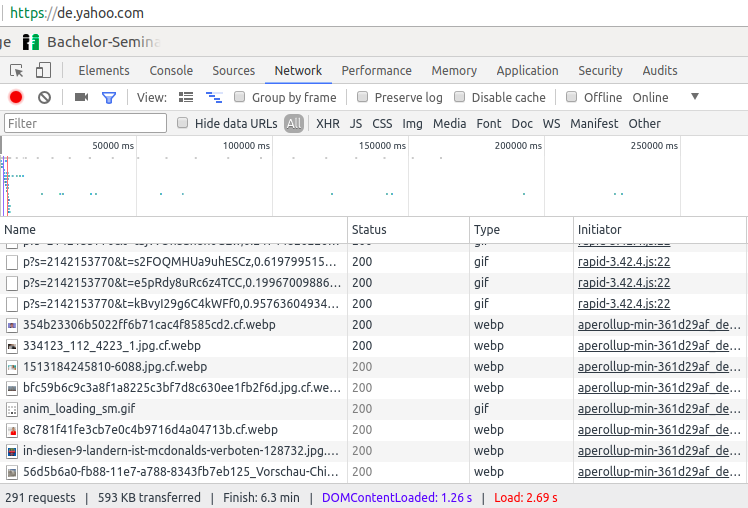
\includegraphics[width=\columnwidth]{yahooRequests}
\caption{Aufrufen von https://de.yahoo.com am 19.02.2018 im Browser Chromium. Links unten sieht man die Anzahl der Anfragen.}
\label{fig:yahoo}
\end{figure}


In der Protokollversion 0.9 gibt es pro Anfrage-Antwort-Paar nur eine TCP-Verbind"-dung. Die Verbindung wird für eine Anfrage geöffnet und nach der Über-tragung der Antwort geschlossen. Das Öffnen und Schließen einer TCP-Verbind"-dung ist ein Overhead. Um ihn zu entfernen wurden in HTTP/1.1 persistente Verbindungen eingeführt. Auf einer persistenten Verbindung kann man eine zweite Anfrage versenden ohne die Antwort auf die erste Anfrage abzuwarten. Das nennt der RFC 2616 Pipelining. Pipelining ist in Abbildung 2 dargestellt.

\begin{figure}[!ht]
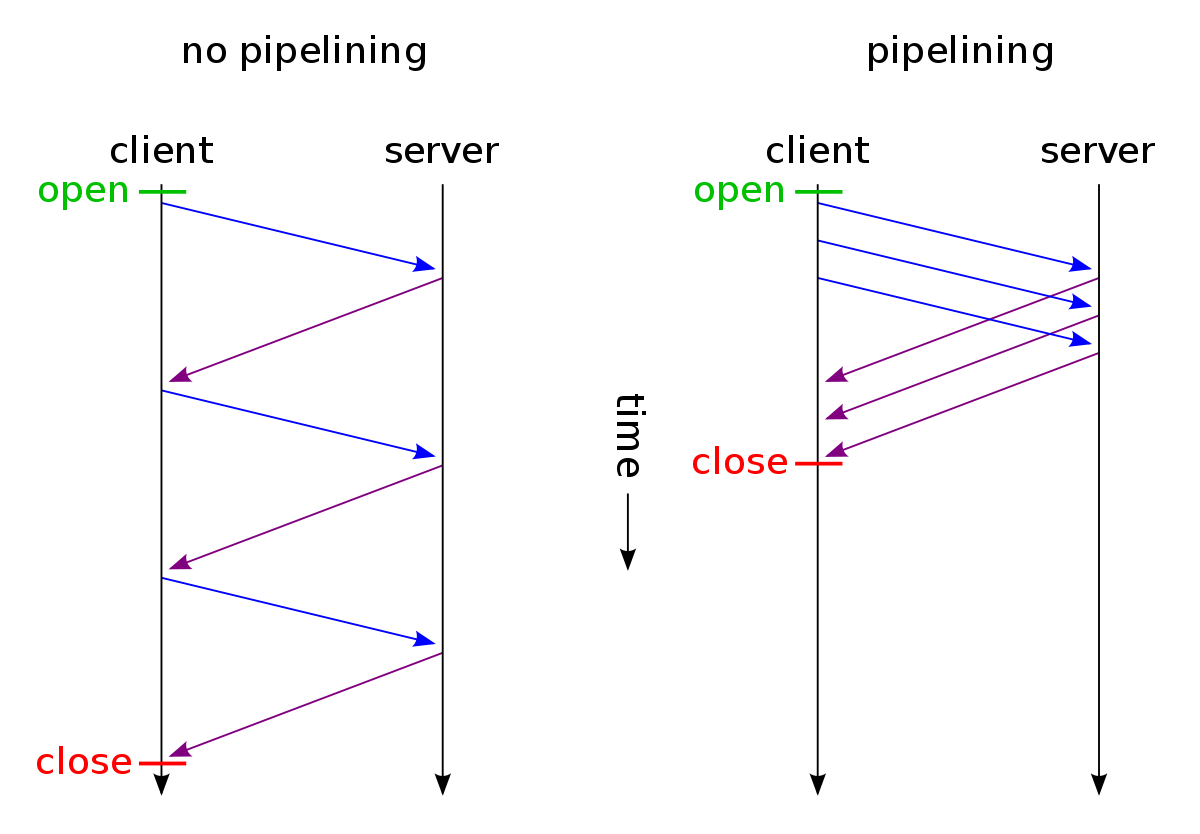
\includegraphics[width=\columnwidth]{1200px-HTTP_pipelining2}
\caption{Pipelining erlaubt es eine Anfrage zu senden, ohne auf die Antwort der vorhergehenden Anfrage zu warten.\cite{Pipelining}}
\end{figure}

Wenn mehrere Anfragen in einer Pipeline auf einer TCP-Verbind"-dung stehen, werden die Anfragen nacheinander abgearbeitet. Eine Anfrage deren Bearbeitung lange dauert kann die Bearbeitung der Anfragen dahinter verzögern. Dieses Phänomen heißt Head-of-Line-Blocking oder HOL-Blocking. Wenn auf einer TCP-Verbind"-dung HOL-Blocking auftritt, kann eine neue Verbindung zum Server geöffnet werden, um neue Requests zu verschicken. Auf der neuen Verbin-dung kann wieder HOL-Blocking auftreten. Da die Anzahl der TCP-Verbind"-dungen zwischen Client und Server begrenzt ist, können alle Verbindungen durch HOL-Blocking blockiert werden. HOL-Blocking ist ein Hindernis, dass die Ladezeit einer Website erheblich beeinträchtigen kann.

Um diesem Problem zu begegnen, wurde in HTTP/2 Multiplexing eingeführt. Multiplexing erlaubt es mehrere Antwort-Anfrage-Paare nebenläufig auf einer TCP-Verbind"-dung zu versenden. Dafür werden Streams verwendet.
Ein Stream ist eine unabhängige, bidirektionale Sequenz von Frames, die zwischen Client und Server in einer HTTP/2-Verbindung ausgetauscht werden \cite{Belshe2015}.
Ein Frame ist die Grundeinheit in die Pakete nach HTTP/2 aufgeteilt werden. In HTTP/2 können Header und Payload eines Pakets in getrennten Frames versendet werden. Um die Frames dem selben Paket zuzuordnen, hat jeder Frame einen Stream Identifier. Der Stream Identifier macht es möglich, dass die Bearbeitungsreihenfolge von Anfragen nicht die Reihenfolge sein muss in der sie gesendet wurden. Das ist die Eigenschaft von Streams, die HOL-Blocking umgeht. Wenn die Bearbeitung eines Frames lange dauert, kann auf der selben TCP-Verbind"-dung ein Frame eines anderen Streams verschickt werden. Das heißt Interleaving. Interleaving ist in Abbildung \ref{Multiplexing} dargestellt.

\section{Zusammenfassung}
HTTP ist ein Request-Response-Protokoll, das zum Datenaustausch zwischen Computern über ein Rechnernetz genutzt wird. Es wurde ursprünglich für ein Dokumentationssystem entwickelt, das den Austausch digitaler Dokumente zwischen Rechnern mit verschiedenen Betriebssystemen ermöglichen sollte. Dieses Dokumentationssystem hat sich zum World Wide Web entwickelt. 
HTTP kommt zum Einsatz, wenn ein Browser eine Internetseite von einem Server anfragt.\newline Ein HTTP-Paket enthält eine Methode, Metadaten und einen Payload. Die Methode drückt die Handlung aus, die der Client vom Server erwartet. Metadaten in HTTP-Paketen sind Header und Statuscodes. Der Payload ist eine Datei, die der Client zum Server übertragen will oder vom Server anfragt. \newline
HTTP baut auf dem Transportprotokoll TCP auf.
Die Verwendung von TCP-Verbind"-dungen hat großen Einfluss darauf wie schnell eine Internetseite angezeigt werden kann. Die Verwendung der TCP-Verbind"-dungen hat sich vom Öffnen und Schließen einer Verbindung für jede HTTP-Anfrage über persistente Verbindungen mit Pipelining zum Multiplexing entwickelt. \newline
HOL-Blocking bedeutet, dass die Bearbeitung eines Pakets in einer Pipeline die Bearbeitung der folgenden Pakete blockiert. Auf Ebene von HTTP-Paketen wurde HOL-Blocking in HTTP/2 mit Multiplexing gelöst.
 Auf der Ebene von TCP-Paketen gibt es auch HOL-Blocking. Dafür entwickelt Google ein alternatives Protokoll unter dem Namen QUIC.
 \begin{figure}[!ht]
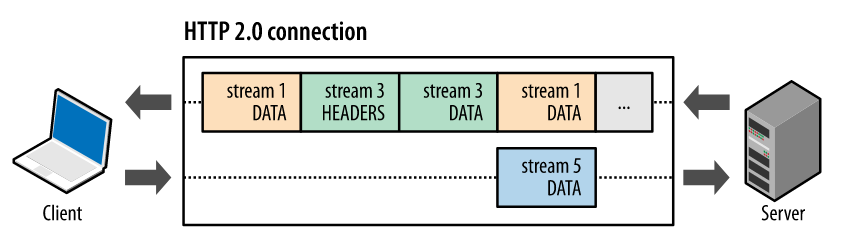
\includegraphics[width=\columnwidth]{Multiplexing.png}
\caption{Interleaving: Mehrere Frames, die durcheinander auf einer TCP-Verbind"-dung verschickt werden. Jeder Frame hat einen Stream Identifier. 
\cite{Interleaving}
}
\label{Multiplexing}
\end{figure}


\bibliographystyle{acm}
\bibliography{literature}


\end{document}

              
 

